\section{Rolling Road}
The Rolling Road is a dynamometer designed to measure the energy conversion efficiency  between the electric energy from AU2's battery and the delivered rotanional energy in the wheel.

\subsection{BDD}
The Block Definition Diagram in \ref{fig:RR_BDD} gives a general overview of the structure of the system.

%The system is made up by a Roll which spins the DC Generator in order to create a voltage drop. The Roll is part of a Load System which able to change the rotational resistance in the Roll.
%Sensors in the system gather data about the power and torque delivered to the system. These sensors are able to send the gathered data to a Computer where it is represented graphically through a GUI. The communication between the system and the Computer is done by a Control Unit.

\begin{figure}[H]
	\centering
	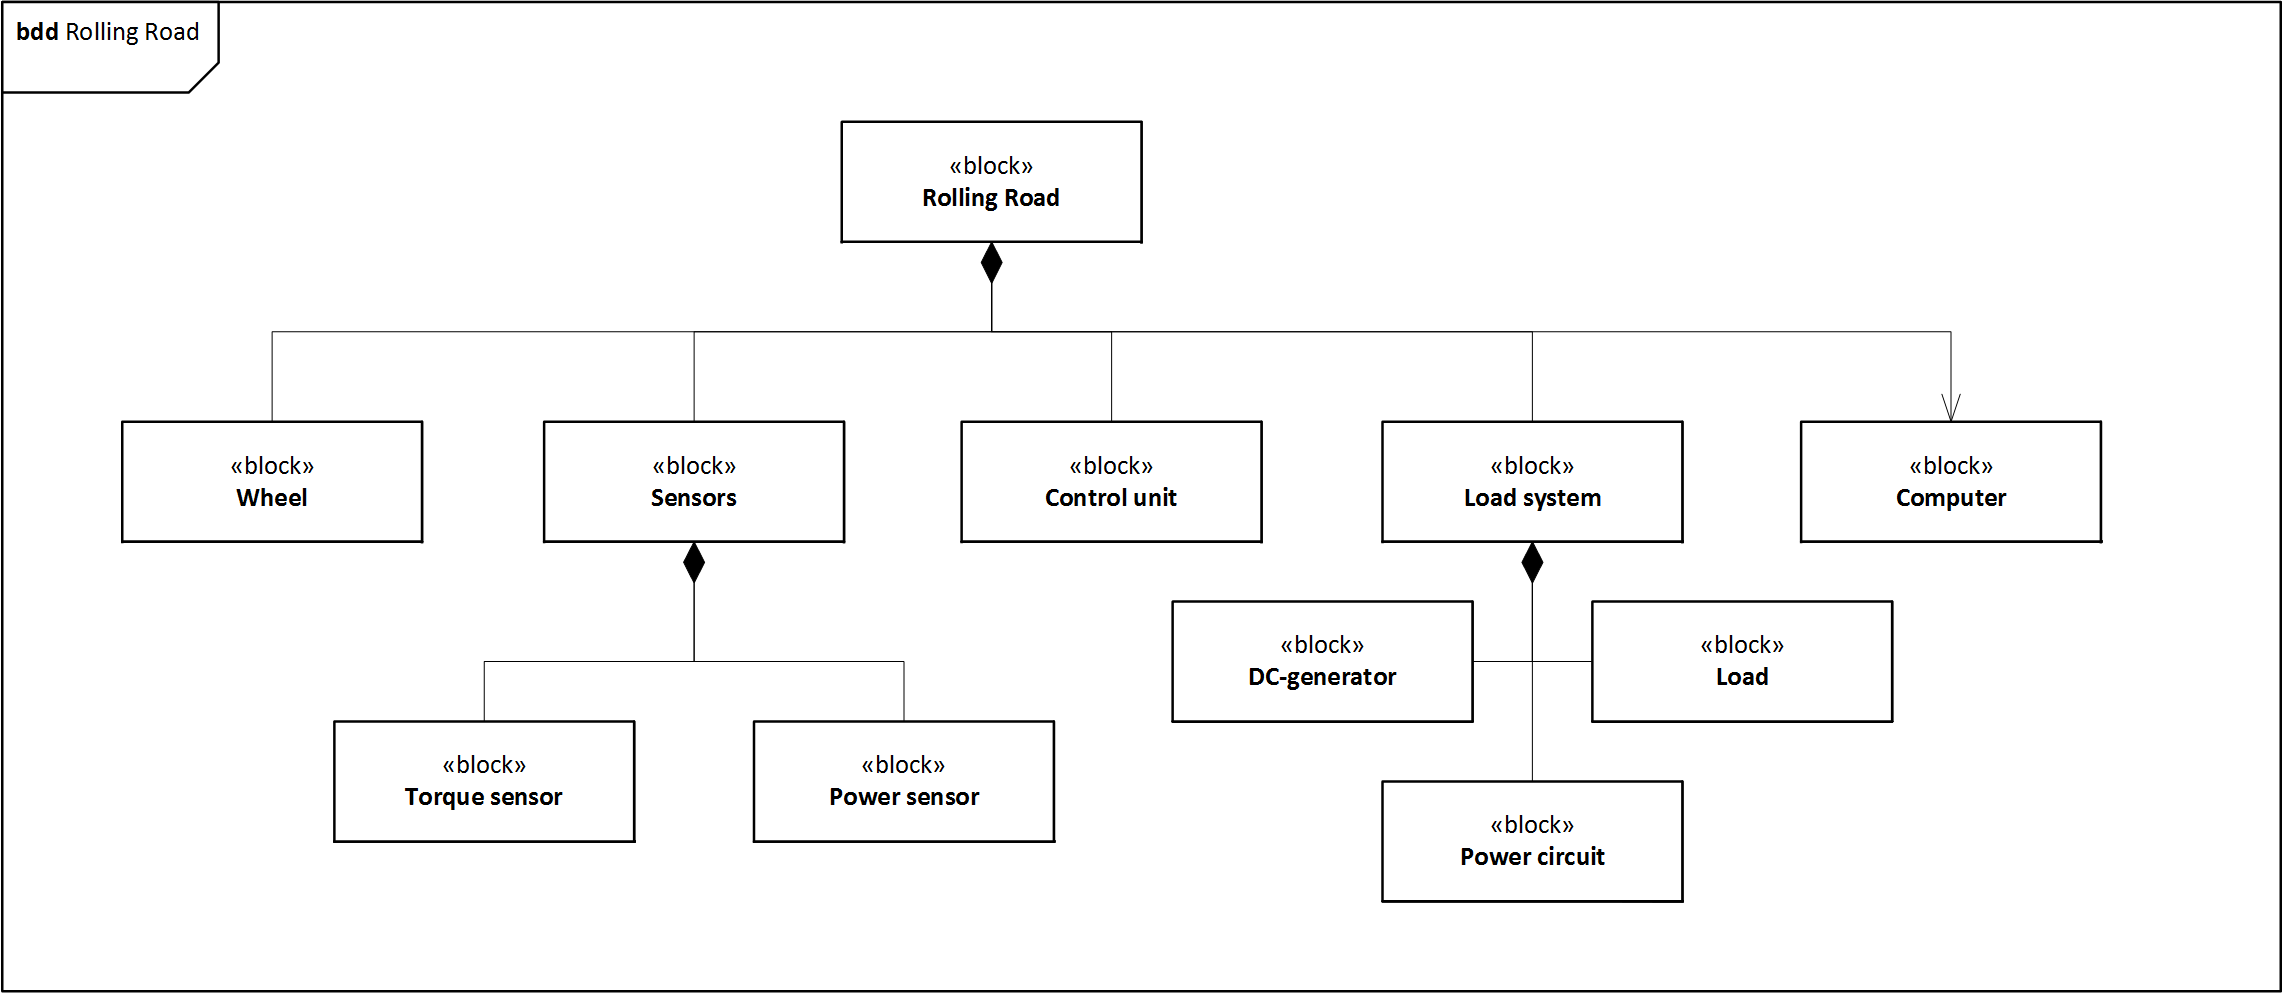
\includegraphics[width=0.9\linewidth]{Architecture/BDD_RollingRoad}
	\caption{BDD for Rolling Road}
	\label{fig:RR_BDD}
\end{figure}

\subsection{Block Description}
The blocks in the BDD are described as follows:

\begin{itemize}
	\item \textbf{Voltage Adaptor}\\
	Description: This block converts 230 VAC to 12 VDC in order to control the system. This allows the system to be directly powered by the mains electricity.
	\item \textbf{Roll Stand}\\
	Description: This block contains the various mechanical subsystems.
	\begin{itemize}
	   	\item \textbf{Roll}\\
	   	Description: The cylinder which is rotated by the vehicle.
	   	\item \textbf{Generator}\\
	   	Description: A DC-generator which generates a voltage proportional to the angular velocity.
	   	\item \textbf{Torque Sensor}\\
	   	Description: Converts the angular velocity and torque to electrical signals.
	\end{itemize}
	\item \textbf{Computer}\\
	Description: Reads values from the Control Unit and displays the data on a GUI.
	\item \textbf{Control Unit}\\
	Description: Reads the Roll's angular velocity, torque, electrical power in the battery and mechanical power given to the Roll. Furthermore it controls the resistance in the Load System and sends the collected data to the Computer.
	\item \textbf{Electrical Circuit}\\
	Description: This block contains the various electrical subsystems.
	\begin{itemize}
		\item \textbf{Signal Converter}\\
		Description: Converts the generated signals from the Torque Sensor to signals which are readable for the Control Unit.
		\item \textbf{Level Converter}\\
		Description: Converts the 12 VDC voltage to 5 VDC in order to power the control unit.
		\item \textbf{Power Sensor}\\
		Description: Converts electrical power from the vehicle's battery to signals which are readable for the Control Unit.
	\end{itemize}
	\item \textbf{Load System}\\
	Description: A seperate electrical circuit which serves as a mechanical resistance in the generator.
\end{itemize}

\subsection{IBD}
The Internal Block Diagram in \ref{fig:RR_IBD} gives a general overview of the system's external connections as well as the internal communication between the blocks in the system.

The system has three external connections: A voltage supplied by the 230 VAC mains, the mechanical power delivered by the vehicle's wheel and the electrical power delivered by the vehicle's battery.

%The Roll rotates as the wheels from the AU2 delivers torque to the system. The torque from the spinning wheel is fed to a Torque Sensor and the Load System through a drive shaft which spins the DC Generator and generates a voltage in the Power Circuit. The voltage is measured by the Control Unit which is also able to control the Load System with a PWM-signal.\\
%Furthermore, the Control System measures the power from AU2's battery and the power delivered to Rolling Road through the Power Sensor and Torque Sensor. The communication with the Computer is done by UART.

\begin{figure}[H]
	\centering
	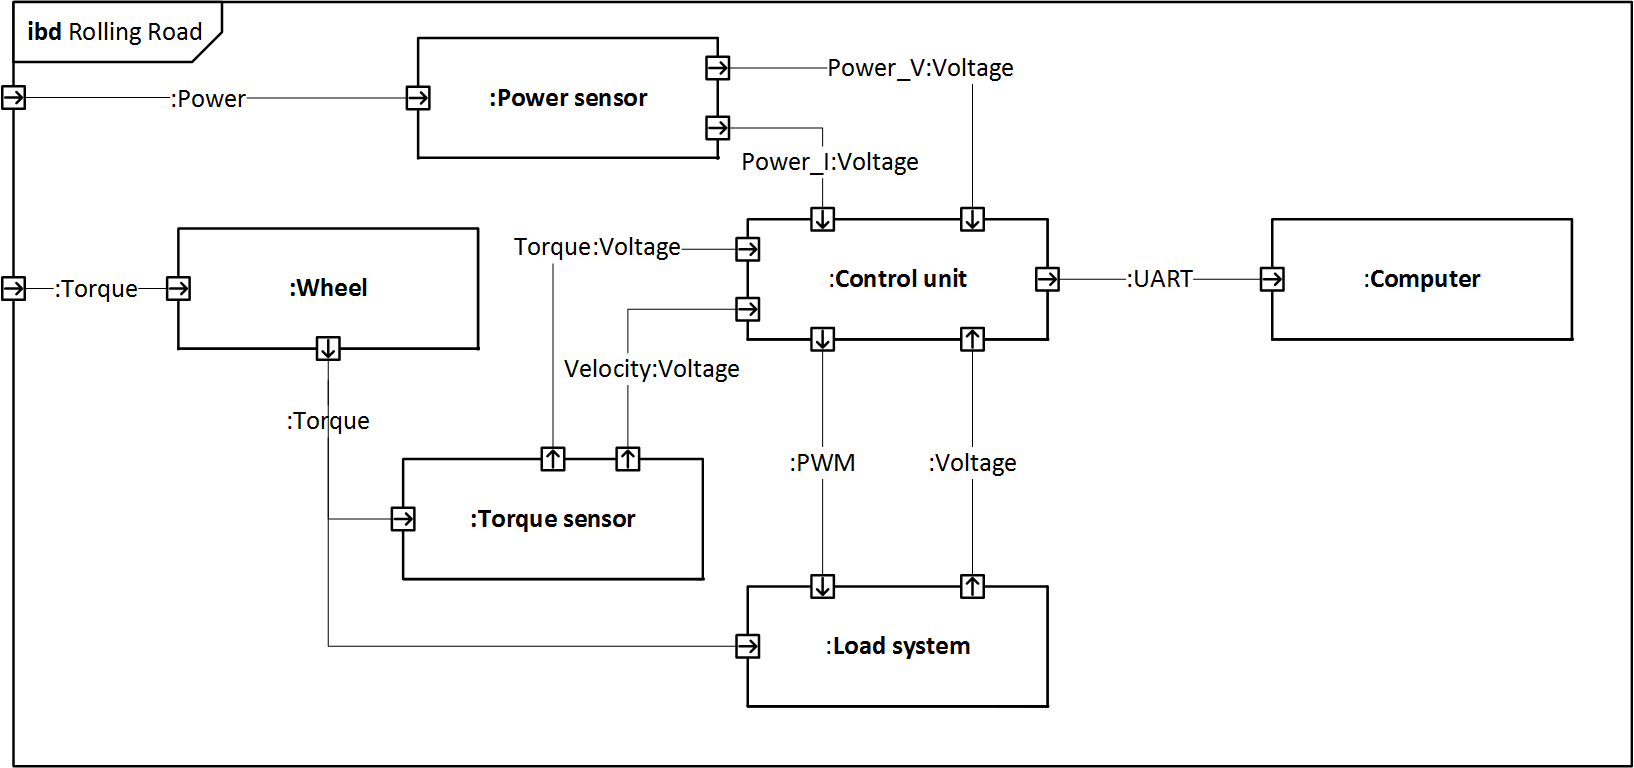
\includegraphics[width=0.9\linewidth]{Architecture/IBD_RollingRoad}
	\caption{IBD for Rolling Road}
	\label{fig:RR_IBD}
\end{figure}

\subsection{Signal description}
The signals and protocols used to communicate between the blocks in Rolling Road are specified in this section.

\textbf{Block :Rolling Road}\\
Block interface description:
\begin{itemize}
	\item \textbf{Supply230:Voltage}\\
	Direction: [External] $\rightarrow$ [Voltage Adaptor]\\
	Description: Voltage from the 230 VAC electrical mains.
	\item \textbf{ExternalMec:Power}\\
	Direction: [External] $\rightarrow$ [Roll]\\
	Description: Mechanical power from the vehicle's wheel.
	\item \textbf{ExternalEl:Power}\\
	Direction: [External] $\rightarrow$ [Power Sensor]\\
	Description: Electrical power from the vehicle's battery.
\end{itemize}

\textbf{Block :Voltage Adaptor}\\
Block interface description:
\begin{itemize}
	\item \textbf{Supply230:Voltage}\\
	Direction: [External] $\rightarrow$ [Voltage Adaptor]\\
	Description: Voltage from the 230 VAC electrical mains.
	\item \textbf{Supply12:Voltage}\\
	Direction: [Voltage Adaptor] $\rightarrow$ [Level Converter] \& [Torque Sensor]\\
	Description: Converted supply voltage of 12 VDC.
\end{itemize}

\textbf{Block :Level Converter}\\
Block interface description:
\begin{itemize}
	\item \textbf{Supply12:Voltage}\\
	Direction: [Voltage Adaptor] $\rightarrow$ [Level Converter]\\
	Description: Converted supply voltage of 12 VDC.
	\item \textbf{Supply5:Voltage}\\
	Direction: [Level Converter] $\rightarrow$ [Load System] \& [Control Unit]\\
	Description: Converted supply voltage of 5 VDC.
\end{itemize}

\textbf{Block :Torque Sensor}\\
Block interface description:
\begin{itemize}
	\item \textbf{Supply12:Voltage}\\
	Direction: [Voltage Adaptor] $\rightarrow$ [Torque Sensor]\\
	Description: Converted supply voltage of 12 VDC.
	\item \textbf{InternalMec:Power}\\
	Direction: [Roll] $\rightarrow$ [Torque Sensor]\\
	Description: Mechanical power given by the rotation of the Roll.
	\item \textbf{Torque:Voltage}\\
	Direction: [Torque Sensor] $\rightarrow$ [Signal Converter]\\
	Description: An analog signal (-5 V to 5 V) which is proportional to the torque measured by the sensor (-5 Nm to 5 Nm).
	\item \textbf{Angle:Frequency}\\
	Direction: [Torque Sensor] $\rightarrow$ [Signal Converter]\\
	Description: A square-wave signal with a frequency which is proportional to the angular velocity measured by the sensor.
\end{itemize}


\textbf{Block :Roll}\\
Block interface description:
\begin{itemize}
	\item \textbf{ExternalMec:Power}\\
	Direction: [External] $\rightarrow$ [Roll]\\
	Description: Mechanical power from the vehicle's wheel.
	\item \textbf{InternalMec:Power}\\
	Direction: [Roll] $\rightarrow$ [Torque Sensor] \& [Generator]\\
	Description: Mechanical power given by the rotation of the Roll.
\end{itemize}

\textbf{Block :Generator}\\
Block interface description:
\begin{itemize}
	\item \textbf{InternalMec:Power}\\
	Direction: [Roll] $\rightarrow$ [Generator]\\
	Description: Mechanical power given by the rotation of the Roll.
	\item \textbf{CEMF:Voltage}\\
	Direction: [Generator] $\rightarrow$ [Load System]\\
	Description: Generated counter electromotive force.
\end{itemize}

\textbf{Block :Signal Converter}\\
Block interface description:
\begin{itemize}
	\item \textbf{Torque:Voltage}\\
	Direction: [Torque Sensor] $\rightarrow$ [Signal Converter]\\
	Description: An analog signal (-5 V to 5 V) which is proportional to the torque measured by the sensor (-5 Nm to 5 Nm).
	\item \textbf{Angle:Frequency}\\
	Direction: [Torque Sensor] $\rightarrow$ [Signal Converter]\\
	Description: A square-wave signal with a frequency which is proportional to the angular velocity measured by the sensor.
	\item \textbf{TorqueC:Voltage}\\
	Direction: [Signal Converter] $\rightarrow$ [Control Unit]\\
	Description: An analog signal (0-5 V) which is proportional to the input signal (Torque:Voltage). This signal can be read by the control unit.
	\item \textbf{AngleC:Frequency}\\
	Direction: [Signal Converter] $\rightarrow$ [Control Unit]\\
	Description: A square-wave signal with an identical frequency as the input signal (Angle:Frequency); but without overshoots. This signal can be read by the control unit.
\end{itemize}

\textbf{Block :Load System}\\
Block interface description:
\begin{itemize}
	\item \textbf{Supply5:Voltage}\\
	Direction: [X] $\rightarrow$ [Y]\\
	Description: Converted supply voltage of 5 VDC.
	\item \textbf{CEMF:Voltage}\\
	Direction: [Generator] $\rightarrow$ [Load System]\\
	Description: Generated counter electromotive force.
	\item \textbf{RegControl:PWM}\\
	Direction: [Control Unit] $\rightarrow$ [Load System]\\
	Description: PWM-signal which controls the size of the load.
	\item \textbf{ISense:Voltage}\\
	Direction: [Load System] $\rightarrow$ [Control Unit]\\
	Description: A voltage which is proportional to the current in the Load System.
\end{itemize}

\textbf{Block :Power Sensor}\\
Block interface description:
\begin{itemize}
	\item \textbf{ExternalEl:Power}\\
	Direction: [External] $\rightarrow$ [Power Sensor]\\
	Description: Electrical power from the vehicle's battery.
	\item \textbf{VoltageP:Voltage}\\
	Direction: [Power Sensor] $\rightarrow$ [Control Unit]\\
	Description: The voltage-drop over the vehicle's battery.
	\item \textbf{CurrentP:Voltage}\\
	Direction: [Power Sensor] $\rightarrow$ [Control Unit]\\
	Description: An analog signal which is proportional to the current delivered by the vehicle's battery.
\end{itemize}

\textbf{Block :Control Unit}\\
Block interface description:
\begin{itemize}
	\item \textbf{Supply5:Voltage}\\
	Direction: [X] $\rightarrow$ [Y]\\
	Description: Converted supply voltage of 5 VDC.
	\item \textbf{TorqueC:Voltage}\\
	Direction: [Signal Converter] $\rightarrow$ [Control Unit]\\
	Description: An analog signal (0-5 V) which is proportional to the input signal (Torque:Voltage). This signal can be read by the control unit.
	\item \textbf{AngleC:Frequency}\\
	Direction: [Signal Converter] $\rightarrow$ [Control Unit]\\
	Description: A square-wave signal with an identical frequency as the input signal (Angle:Frequency); but without overshoots. This signal can be read by the control unit.
	\item \textbf{RegControl:PWM}\\
	Direction: [Control Unit] $\rightarrow$ [Load System]\\
	Description: PWM-signal which controls the size of the load.
	\item \textbf{ISense:Voltage}\\
	Direction: [Load System] $\rightarrow$ [Control Unit]\\
	Description: A voltage which is proportional to the current in the Load System.
	\item \textbf{VoltageP:Voltage}\\
	Direction: [Power Sensor] $\rightarrow$ [Control Unit]\\
	Description: The voltage-drop over the vehicle's battery.
	\item \textbf{CurrentP:Voltage}\\
	Direction: [Power Sensor] $\rightarrow$ [Control Unit]\\
	Description: An analog signal which is proportional to the current delivered by the vehicle's battery.
	\item \textbf{:UART}\\
	Direction: [Control Unit] $\rightarrow$ [Computer]\\
	Description: A signal which transmits data to the computer using the UART-protocol.
\end{itemize}

\textbf{Block :Computer}\\
Block interface description:
\begin{itemize}
	\item \textbf{:UART}\\
	Direction: [Control Unit] $\rightarrow$ [Computer]\\
	Description: A signal which transmits data to the computer using the UART-protocol.
\end{itemize}